% !TeX spellcheck = de_AT_frami
\section{Interpolation}
	\begin{enumerate}
		\item \textbf{Wie werden die dividierten Differenzen berechnet?} \\
			Mit Hilfe eines Differenzenschema oder Differenzentableau. \\
			Allgemeines Differenzenschema für 5 Punkte
				\begin{align*}
				\begin{array}{cc|cccc}
					x_i & y_i &              \delta y_i              &                     \delta^2 y_i                     &                       \delta^3 y_i                       &                       \delta^4 y_i                       \\ \hline
					x_0 & y_0 &  \\
					    &     & \delta y_0 = \frac{y_1-y_0}{x_1-x_0} &  \\
					x_1 & y_1 &                                      & \delta^2 y_0 = \frac{\delta y_1-\delta y_0}{x_2-x_0} &  \\
					    &     & \delta y_1 = \frac{y_2-y_1}{x_2-x_1} &                                                      & \delta^3 y_0 = \frac{\delta^2 y_1-\delta^2 y_0}{x_3-x_0} &  \\
					x_2 & y_2 &                                      & \delta^2 y_1 = \frac{\delta y_2-\delta y_1}{x_3-x_1} &                                                          & \delta^4 y_0 = \frac{\delta^3 y_1-\delta^2 y_0}{x_4-x_0} \\
					    &     & \delta y_2 = \frac{y_3-y_2}{x_3-x_2} &                                                      & \delta^3 y_1 = \frac{\delta^2 y_2-\delta^2 y_1}{x_4-x_1} &  \\
					x_3 & y_3 &                                      & \delta^2 y_2 = \frac{\delta y_3-\delta y_2}{x_4-x_2} &  \\
					    &     & \delta y_3 = \frac{y_4-y_3}{x_4-x_3} &  \\
					x_4 & y_4 &
				\end{array}
			\end{align*}
		\item \textbf{Wie ist das Newtonsche Interpolationspolynom definiert?}
			\begin{align*}
				p(x)=y_0+(x-x_0)\delta y_0+(x-x_0)(x-x_1)\delta^2 y_0+\dots+(x-x_0)(x-x_1)\cdots(x-x_{n-1}) \delta^\text{n} y_0
			\end{align*}
		
		\item \textbf{Wie wird mit dem Hornerschema ein Polynom $\mathbf{p(x)=a_0+a_1x+\dots +a_nx^n}$ ausgewertet?} \\
			\begin{align*}
				p(x)=a_0+x(a_1+x(a_2+\cdots+x(a_{n-2}+x(a_{n-1}+x\,a_n))\cdots))
			\end{align*}
		\item \textbf{Wie wird mit dem Hornerschema ein Newtonsches Interpolationspolynom ausgewertet?}
			\begin{figure}[htbp]
				\centering
				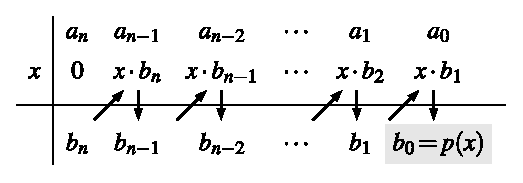
\includegraphics[width=0.45\linewidth]{Kap3_1}
			\end{figure}
		\item \textbf{Wie sind die Lagrange-Polynome definiert? Welche Eigenschaften haben sie?}
			\begin{align*}
				\ell_i(x)&=\frac{(x-x_0)(x-x_1)\cdots\reallywidehat{(x-x_i)}\cdots(x-x_n)}{(x_i-x_0)(x_i-x_1)\cdots\reallywidehat{(x_i-x_i)}\cdots(x_i-x_n)} \\
				\ell_i(x_j)&=\delta_{ij} =
					\begin{cases}
						1, & \text{falls } i=j,\\
						0, & \text{falls } i\neq j.
					\end{cases} \nonumber
			\end{align*}
			Wobei die überdachten Terme wegzulassen sind.
		\item \textbf{Wie wird mit Hilfe der Lagrange-Polynome das Langrangesche Interpolationspolynom berechnet?}
			\begin{align*}
				p(x)=\sum_{i=0}^{n}y_i\,\ell_i(x), \quad p(x_j)=y_j
			\end{align*}
		
		\pagebreak
		
		\item \textbf{Erklären Sie die Begriffe Datenfehler, Verstärkungsfaktor, Lebesgue-Funktion und Lebesgue-Konstante in Zusammenhang mit der Polynominterpolation. Was ist die Kondition der Polynominterpolation?} \\
			An einer Stützstelle \(x_j\) kann ein Datenfehler \(\varepsilon_j\) auftreten.
			Führt man diesen in ein Lagrange-Polynom ein erhält man
			\begin{align*}
				\overline{p}(x)=\sum_{i=0}^{j-1}\left( y_i\,\ell_i(x)\right) + (y_j+\varepsilon_j)+\sum_{i=j+1}^{n}\left( y_i\,\ell_i(x)\right).
			\end{align*}
			Der Fehler \(\varepsilon_i\) wird also um den Faktor  \(\abs{\ell_i}\) verstärkt.
			Wenn alle Knoten mit Fehlern verseht sind ergibt sich
			\begin{align*}
				\overline{p}(x)=p(x)+\sum_{i=0}^{n}\left( \varepsilon_i\,\ell_i \right) .
			\end{align*}
			Falls die einzelnen Fehler durch \(\varepsilon_i\le\text{M}\) beschränkt sind erhält man für den absoluten Fehler die Abschätzung
			\begin{align*}
				\underbrace{\abs{\overline{p}(x)-p(x)}}_\text{abs. Fehler Output}\leq \text{M}\underbrace{\sum_{i=0}^{n}\overbrace{\abs{\ell_i(x)}}^{\kappa_{\text{abs},i}(x)}}_{\kappa_\text{abs}(x)}
				= \text{M}\cdot\kappa_\text{abs}(x).
			\end{align*}
			Wobei \(\kappa_{\text{abs},i}=\abs{\ell_i(x)}\) der Verstärkungsfaktor für den Datenfehler in der Stützstelle \(i\) und die Lebesgue-Funktion \(\kappa_\text{abs}=\lambda_n(x)=\sum_{i=0}^{n}|\ell_i(x)|\) die absolute Kondition für die Polynominterpolation ist. Die schlechteste Konditionszahl \(\lambda_n(x)\) im Intervall \([\text{min}_ix_i,\text{max}_ix_i]\) nennen wir Lebesgue-Konstante und erhalten sie durch
			\begin{align*}
				\underset{x\in[\text{min}_ix_i,\text{max}_ix_i]}{\text{max}} \lambda_n(x):=\Lambda_n.
			\end{align*}
		\item \textbf{Was besagt der Satz über den Fehler des Interpolationspolynoms? Wie ist der Verfahrensfehler definiert?} \\
			Gegeben seien \(n+1\) verschiedene Stützstellen \(x_i, i=0,\dots,n\), in einem Intervall \([a,b]\) und eine \(n+1\)-mal stetig differenzierbare Funktion \(f\in\mathscr{C}^{n+1}([a,b])\). Dann gilt für den Fehler \( f(x)-p(x) \) des Interpolationspolynoms folgende Aussage: \\
			Für alle \( x\in[a,b] \) gibt es ein \( \xi=\xi(x) \), das also von x abhängen kann, mit
			\begin{align*}
				\xi \in \left( \text{min}\{x_0,\dots,x_n,x \}, \text{max}\{x_0,\dots,x_n,x \} \right)
			\end{align*}
			sodass gilt:
			\begin{align*}
				f(x)-p(x)=(x-x_0)(x-x_1)\cdots(x-x_n)\frac{f^{(n+1)\left(\xi\right)}}{(n+1)!}.
			\end{align*}
			Somit ergibt sich für den Verfahrensfehler
			\begin{align*}
				\prod(x):=\abs{(x-x_0)(x-x_1)\cdots(x-x_n)}.
			\end{align*}
			
		\pagebreak
			
		\item \textbf{Wie sind die Tschebyscheff-Polynome definiert? Welche Eigenschaften haben sie?} \\
			Die durch Abbildung \(T_n:[-1,1]\rightarrow[-1,1]\) mit
			\begin{align*}
				T_n(x)=\cos(n\arccos(x))
			\end{align*}
			definierten Polynome heißen Tschebyscheff-Polynome. Für sie gilt:
			\begin{enumerate}
				\item[(1)] \(T_n\) ist ein Polynom \(n\)-ten Grades in \(x=\cos\phi\).
				\item[(2)] Rekursionsformel für Tschebyscheff-Polynome:\\
						\(T_0(x)=1, T_1(x)=x\) und \(T_{n+1}(x)=2xT_n(x)-T_{n-1}(x),\,\, n=1,2,\dots\)
				\item[(3)] \(T_n(x)\leq1\) für \(x\in[-1,1] \).
				\item[(4)] \(T_n\) ist eine gerade oder ungerade Funktion, je nachdem, ob n gerade oder ungerade ist.
				\item[(5)] \(T_n\) besitzt ganzzahlige Koeffizienten. Der führende Koeffizient ist \(2^{n-1}\) für \(n\geq1\).
				\item[(6)] \(T_n\) nimmt für \(n\geq 1\) im Intervall \([-1,1]\) (n+1)-mal die Werte \(\pm1\) an, nämlich für \(x=\cos\frac{k\pi}{n},k=0,1,\dots,n\). Insbesondere gilt \(T_n(1)=1, T_n(-1)=(-1)^n\).
				\item[(7)] \(T_n\) hat \(n\) reelle Nullstellen in \([-1,1]\), nämlich die Tschebyscheff-Knoten
					\begin{align*}
						t_k^{(n)}=\cos\left( \frac{2k-1}{2n}\pi \right),\, k=1,\dots,n. 
					\end{align*}
				\item[(-)] Minmax-Eigenschaft: Gegeben seien \(n+1\) verschiedene Stützstellen \(x_i, i=0,\dots,n\) im Intervall \([-1,1]\). Die Maximumsnorm des Verfahrensfelher
				\begin{align*}
					\norm{\prod(x)}_\infty=\underset{x\in[-1,1]}{\max}\abs{(x-x_0)(x-x_1)\cdots(x-x_n)}
				\end{align*}
				nimmt einen minimalen Wert an, falls \(x_0,x_1,\dots,x_n\) die Nullstellen von \(T_{n+1}(x)\) sind.
			\end{enumerate}
		\item \textbf{Wie berechnet man die Knoten für die Tschebyscheff-Interpolationspolynome im Intervall \(\mathbf{[−1,1]}\) bzw. \(\mathbf{[a,b]}\)? Welche Vorteile hat die Verwendung von Tschebyscheff-Knoten im Vergleich zu äquidistanten Stützstellen.} \\
			\(T_n\) hat \(n\) reelle Nullstellen in \([-1,1]\), nämlich die Tschebyscheff-Knoten
			\begin{align*}
				t_k^{(n)}=\cos\left( \frac{2k-1}{2n}\pi \right),\, k=1,\dots,n. 
			\end{align*}
			Für \([a,b]\) wird die Transformation
			\begin{align*}
				[-1,1]\rightarrow[a,b], t\rightarrow x(t)=\frac{1}{2}(a+b)+\frac{1}{2}(b-a)t
			\end{align*}
			ausgeführt und man erhält die Tschebyscheff-Knoten in \([a,b]\)
			\begin{align*}
				x_k^{(n)}=\frac{a+b}{2}+\frac{b-a}{2}t_k^{(n)}.\quad t_k^{(n)} \text{ ist } k\text{-ter Tschebyscheff-Knoten in }[-1,1]
			\end{align*}
			Die Tschebyscheff-Interpolation ist wesentlich besser konditioniert.
			
		\item \textbf{Wie lässt sich das dividierte Differenzenschema und das Newtonsche Interpolationspolynom verallgemeinern, falls in den Stützstellen auch noch Ableitungen vorgegeben sind?} \\
			Durch Hermite-Interpolation. Idee: Interpolation durch die Punkte \((x_i,y_i),(x_i+h,y_i+hy_i'),i=0,\dots,n\), und Grenzübergang \(h\rightarrow0\). Führt zu Differenzenschema in dem Punkte doppelt angeschrieben und Werte für die man mit 0 dividieren müsste durch die gegebenen Ableitungen ersetzt werden.
			
		\pagebreak			
		
		\item \textbf{Wie wird mit stückweise konstanten Funktionen interpoliert?} \\
			Das Intervall \([a,b]\) wird in \(n\) Intervalle unterteilt, wobei die Intervallsgrenzen genau zwischen den Knoten liegen. Die Treppenfunktion definiert sich aus den Intervallen \(I_i\) und den Stützstellen \(x_i\) zu
			\begin{align*}
				s(x)=\sum_{i=0}^{n}y_i\,\chi_i(x)
				\intertext{mit}
				\chi_i(x)=\begin{cases}
				1, & \text{falls } x\in I_i,\\
				0, &  sonst.
				\end{cases}
			\end{align*}
			\begin{figure}[htbp]
				\centering
				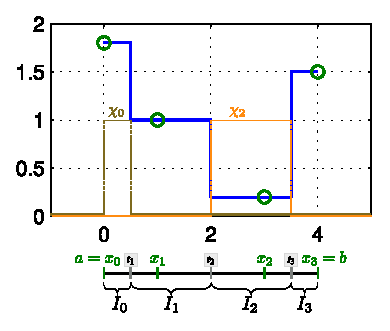
\includegraphics[width=0.4\linewidth]{Kap3_2}
			\end{figure}
		
		\item \textbf{Wie wird mit stetigen, stückweise linearen Funktionen interpoliert?} \\
			Wie oben, nur wird \(\chi_i\) ersetzt durch die Hutfunktion
			\begin{align*}
				\varphi_i=\begin{cases}
					\frac{x-x_{i-1}}{x_i-x_{i-1}}\,\,x\in[x_{i-1},x_i], & \text{falls } i=1,\dots,n \\
					\frac{x_{i+1}-x}{x_{i+1}-x_i}\,\,x\in[x_i,x_{i+1}], & \text{falls } i=0,\dots,n-1 \\
					0, \text{sonst}
				\end{cases}
			\end{align*}
			was analog zu konstanten Funktionen auf
			\begin{align*}
				s(x)=\sum_{i=0}^{n} y_i\,\varphi_i(x)
			\end{align*}
			führt.
			\begin{figure}[htbp]
				\centering
				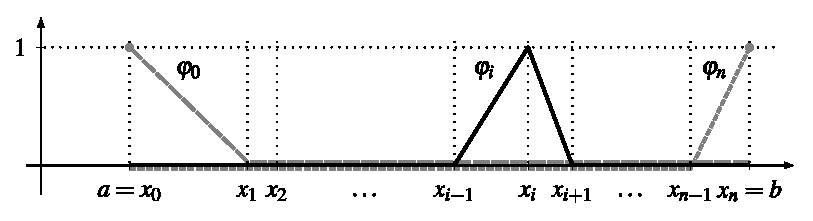
\includegraphics[width=0.6\linewidth]{Kap3_3}
			\end{figure}
				\begin{figure}[htbp]
				\centering
				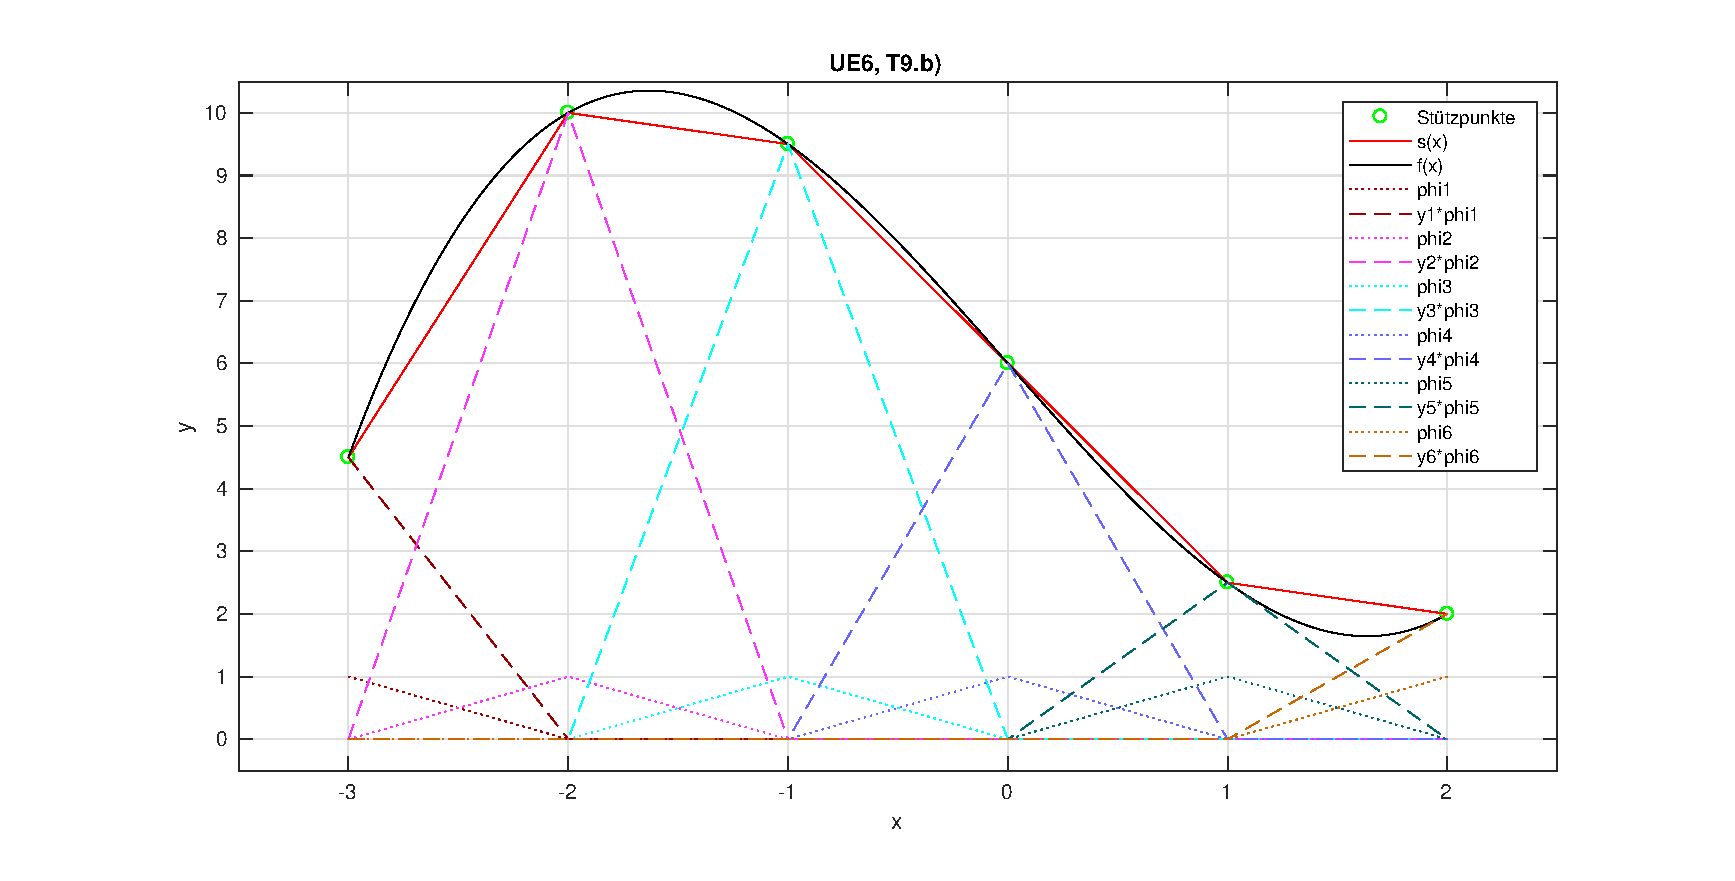
\includegraphics[width=1.0\textwidth]{T9b}
			\end{figure}
		
		\pagebreak
		
		
		\item \textbf{Was sind Hutfunktionen und welche Eigenschaften haben sie?} \\
			Stückweise lineare Funktionen
			\begin{align*}
				\varphi_i=\begin{cases}
							\frac{x-x_{i-1}}{x_i-x_{i-1}}\,\,x\in[x_{i-1},x_i], & \text{falls } i=1,\dots,n \\
							\frac{x_{i+1}-x}{x_{i+1}-x_i}\,\,x\in[x_i,x_{i+1}], & \text{falls } i=0,\dots,n-1 \\
							0, \text{sonst}
						\end{cases}
			\end{align*}
			für die gelten
			\begin{align*}
				\phi_i(x_k)=\delta_{ij}.
			\end{align*}
		\item \textbf{Was für Eigenschaften besitzen kubische Splines? Was für Typen von kubischen Splines gibt es?} \\
			Eigenschaften:
			\begin{itemize}
				\item \(s_i(x_i)=y_i,\,i=0,\dots,n\) (Interpolationsbedingung)
				\item \(s\in\mathscr{C}^2([a,b])\), d.h. zweimal stetig differenzierbar
				\item \(s_i:=\eval[0]{s}_{[x_i,x_{i+1}]} \in \mathbb{P}_3([x_i,x_{i+1}]),\,i=0,\dots,n-1.\)
			\end{itemize}
			Typen:
			\begin{itemize}
				\item Natürlicher Spline \\
					\(s''(x_0)=s''(x_n)=0\) \\
					Die Momente an beiden Enden sind 0.
				\item Eingespannter Spline (vollständiger Spline) \\
					\(s'(x_0)=y_0',\,s'(x_n)=y_n'\) \\
					Die beiden Enden sind eingespannt und die Steigungen vorgegeben.
				\item Periodischer Spline \\
					\( s(x_0)=s(x_n),\,s'(x_0)=s'(x_n),\,s''(x_0)=s''(x_n) \).
				\item Not a knot \\
					\(s'''\) ist stetig in \(x_1\) und \(x_{n-1}\) \\
					Auf den ersten und letzten beiden Intervallen wird ein durchgehendes Polynom dritten Grades verwendet.
			\end{itemize}
		\item \textbf{Wieso ist es besser durch viele Punkte einen kubischen Spline zu legen, statt ein Interpolationspolynom zu verwenden?} \\
			Polynome schaukeln sich am Rand auf und sind daher zur Interpolation ungeeignet, wenn man ein Polynom durch viele Punkte mit beliebigen, paarweise verschiedenen Abszissen legen will.
		
		\item \textbf{Wie wird auf einem rechteckigen Gitter zweidimensional interpoliert?} \\
			Analog zum eindimensionalen Fall benützen wir zwei Lagrange-Polynome
			\begin{align*}
				\ell_i(x)&=\frac{(x-x_0)(x-x_1)\cdots\reallywidehat{(x-x_i)}\cdots(x-x_n)}{(x_i-x_0)(x_i-x_1)\cdots\reallywidehat{(x_i-x_i)}\cdots(x_i-x_n)} \\
				L_j(y)&=\frac{(y-y_0)(y-y_1)\cdots\reallywidehat{(y-y_j)}\cdots(y-y_m)}{(y_j-y_0)(y_j-y_1)\cdots\reallywidehat{(y_j-y_j)}\cdots(y_j-y_m)}
			\end{align*}
			um auf das Interpolationspolynom
			\begin{align*}
				p(x,y)=\sum_{i=0}^{n}\sum_{j=0}^{m}z_{ij}\ell_i(x)L_j(y)
			\end{align*}
			zu kommen, wobei \( \ell_i(x)L_j(y) \) das zur Stützstelle \((x_i,y_j)\) gehörige Lagrange-Polynom ist. Wiederum gilt \linebreak \(l_i(x_i)L_j(y_j)=1\) und \(l_i(x_r)L_j(y_s)=0\) für alle anderen Punkte \((x_r,y_s)\neq(x_i,y_j)\) des Gitters. \\
			Nun kann man entweder primär von links nach rechts und dann von oben nach unten rechnen, oder umgekehrt, hier nur eine Art.\\
			\(p(x,y)\) wird umgeformt zu
			\begin{align*}
				p(x,y)=\sum_{j=0}^{m}\left(\sum_{i=0}^{n}z_{ij}l_i(x)\right)L_j(y)=\sum_{j=0}^{m}r_j(x)L_j(y).
			\end{align*}
			\(r_j(x)\) ist das eindeutige Interpolationspolynom vom Grad \(n\) durch die Punkte \( (x_0,y_i,z_{0j}),\dots,(x_n,y_j,z_{nj})\).
			
			
		\item \textbf{Wie wird die zweidimensionale, stetige, stückweise lineare Interpolierende auf einem rechteckigen Gitter bestimmt?} \\
			Wir betrachten nur ein Rechteck \([x_i,x_{i+1}]\times[y_j,y_{j+1}]\) in dem der Punkt \((x,y)\) liegt.
			\begin{align*}
				s(x,y)=z_{ij}\varphi_i(x)\Phi_j(y)+z_{i+1,i}\varphi_{i+1}(x)\Phi_j(x)+z_{i,j+1}\varphi_i(x)\Phi_{j+1}(y)+z_{i+1,j+1}\varphi_{i+1}(x)\Phi_{j+1}(y)
			\end{align*}
			Wobei \(\varphi_i\) und \(\Phi_j\) die Hutfunktionen in x- und y-Richtung sind.
		
	\end{enumerate}